\documentclass{ctexart}
\usepackage{amsmath}
\usepackage{geometry}
\usepackage{hyperref}
\usepackage{graphicx}
\usepackage{float}
\title{RLC串联电路的暂态过程}
\author{陈启钰\,\,2300011447}
\date{\today}
\begin{document}
	\maketitle
	\section{暂态过程的定义}
	暂态过程是电路从一个稳定状态到另一个稳定状态所经历的过程。
	\section{RC串联电路的暂态过程}
	充电过程
	\begin{align}
		U_C=E\left(1-e^{-\frac{t}{RC}}\right),U_R=Ee^{-\frac{t}{RC}}
	\end{align}
	放电过程
	\begin{align}
		U_C=Ee^{-\frac{t}{RC}},U_R=-Ee^{-\frac{t}{RC}}
	\end{align}
	$U_C$不能跃变,因为其电荷$Q$不能跃变,但是$U_R$可以跃变。
	\section{RC串联电路的时间常数}
	时间常数定义为
	\begin{align}
		\tau=RC
	\end{align}
	实验中通过测量电容两端电压(放电时),测量电容从开始放电到其电压达到最大值的$1/e$所需要的时间,就是时间常数$\tau$。
	\section{RL串联电路的暂态过程}
	电流增长过程
	\begin{align}
		U_L=Ee^{-\frac{R}{L}t},U_R=E\left(1-e^{-\frac{R}{L}t}\right)
	\end{align}
	电流消失过程
	\begin{align}
		U_L=-Ee^{-\frac{R}{L}t},U_R=Ee^{-\frac{R}{L}t}
	\end{align}
	$U_R$不可跃变,因为$I$不能跃变,而$U_L$可以跃变。
	时间常数
	\begin{align}
		\tau=\frac{L}{R}
	\end{align}
	\section{RLC串联电路的暂态过程}
	欠阻尼($R<2\sqrt{\frac{L}{C}}$)
	\begin{align}
		U_C=\frac{1}{\sqrt{1-\frac{CR^2}{4L}}}Ee^{-\frac{t}{\tau}}\cos{(\omega t+\phi)},\tau=\frac{2L}{R},\omega=\frac{1}{\sqrt{LC}}\sqrt{1-\frac{CR^2}{4L}}
	\end{align}
	过阻尼($R>2\sqrt{\frac{L}{C}}$)
	\begin{align}
		U_C=\frac{1}{\sqrt{\frac{CR^2}{4L}-1}}Ee^{-\frac{t}{\tau}}\sinh{(\omega t+\phi)},\tau=\frac{2L}{R},\omega=\frac{1}{\sqrt{LC}}\sqrt{\frac{CR^2}{4L}-1}
	\end{align}
	临界阻尼($R=2\sqrt{\frac{L}{C}}$)
	\begin{align}
		U_C=\left(1+\frac{t}{\tau}\right)Ee^{-\frac{t}{\tau}},\tau=\frac{2L}{R}
	\end{align}
	小阻尼情况下,振荡周期可以直接测量电容电压的各个峰值及其对应的时间,然后计算得到振动的周期。从最大幅度衰减到最大幅度的$1/e$倍的时间即为时间常量的值(也可以通过测量每个极大值振幅然后进行拟合得到)。
	
	为找到临界阻尼状态,可以先调节电阻使电路在欠阻尼状态,然后慢慢调节使得$U_C$的振荡幅度越来越小,直到看不见,此时达到临界阻尼状态。
	\section{实验电路图}
	\begin{figure}[H]
		\centering
		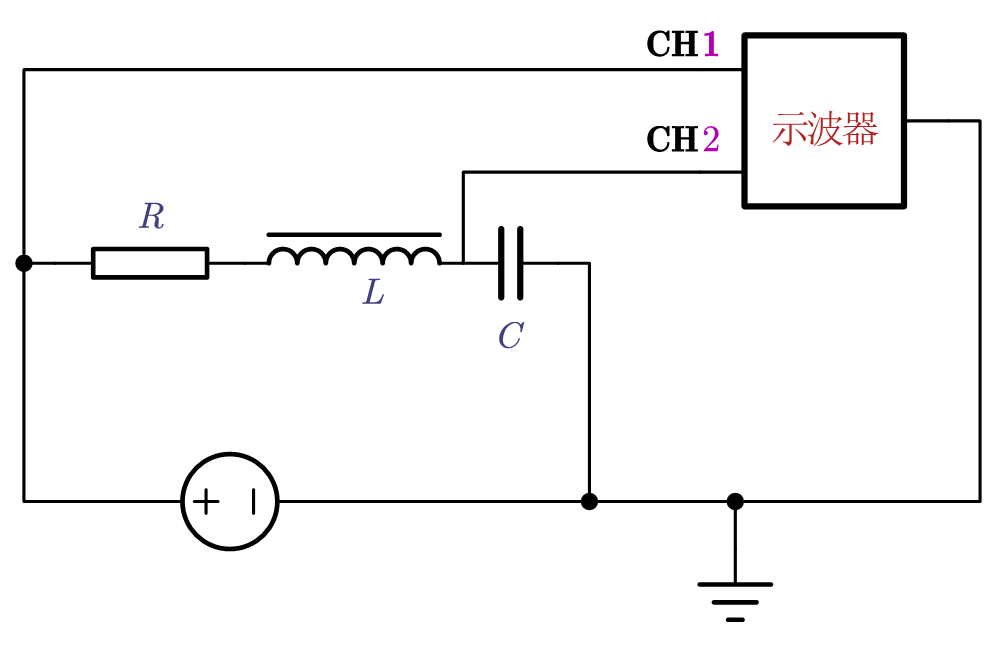
\includegraphics[width=0.6\linewidth]{fig.png}
		\caption{实验电路图}
	\end{figure}
	教材图28-12中,不能直接用CH2通道测量$\text{X}_1$的电压,因为需要保证信号发生器、CH1通道和CH2通道共地。
	\section{关于示波器的若干问题}
	数字储存示波器是对输入信号先进行取样和模数转换,将输入的模拟信号转换为数字量并储存在存储器内,示波器内的微处理器则将存储器内的数字信号转换成可视波形。由于它的存储功能,数字存储示波器特别适合俘获和显示单脉冲信号。但是模拟示波器的输入信号是经过放大直接加到显示器的偏转版上来显示波形,当信号消失时显示屏上的波形也随即消失。
	
	图28-14中,脉冲持续时间约1s,高低电平差约400mV。
	
	750mV表示触发电平。
\end{document}